% !TeX root = ../main.tex
% !TEX root = ../main.tex
% -*- root: ../main.tex -*-
% -*- program: pdflatex -*-
\chapter{前言}

\section{粒子物理学}

物质是由什么组成的?这是人们研究自然界的普遍规律时关心的问题。在《庄子.天下篇》中,庄子有“一尺之捶,日取其半,万世不竭”的观点。说的是有一个一尺长的捶子,每天取它剩下的一半,这样取下去,可以一万世也取不尽。这是古代中国的辩证思想,认为物质的组成是没有极限的。中国夏朝时的“五行学说”认为物质是由金、木、水、火、土组成的。古希腊也有物质有水、火、土和空气等基本元素组成的观点,哲学家~Democritus~的观点是万物的本原是原子和虚空,原子是“不可再分”的。十九世纪初英国的科学家道尔顿提出原子理论。认为,原子是物质世界的最小单元,它是单一的,且独立的,不能被继续分割的,状态在化学变化中是稳定的,同一类型的原子的属性是一致的。这是真正带有近代性质的原子论。十九世纪,自然学科创立并蓬勃发展,物理学、化学等学科相继诞生,通过实验对物质的研究,提出物质都是由不同分子组成的,不同分子的性质上的不同导致物质的物理和化学性质的之间有差异。分子是有原子组成的。门捷列夫提出的元素周期表则告诉我们物质是由~110~多种的不同的元素组成的。二十世纪物理学蓬勃发展,量子力学和相对论相继建立并发展起来,实验上各类粒子相继被发现。例如~1897~年汤普逊发现电子;~1901~年普朗克提出光量子假说,之后的~1905~年爱因斯坦利用此假说成功解释了光电效应;~1911~年卢瑟福提出原子的核式结构,并于~1919~年发现了p;~1932~年查德威克发现了中子;~1932~年发现了第一个反粒子正电子;~1937~年发现~$\mu$~子;~1947~年发现~$\pi$~介子;~1950~年发现~$K$~介子,~$\Lambda$~,~$\Sigma$~;~1955~年发现反质子;~1956~年发现反中子;~1974~年发现~$J/\Psi$~介子,证实了粲(c)夸克的存在;~1975~年发现~$\tau$~轻子;~1983~年发现玻色子:~$W^{\pm}$~和~$Z^{0}$~;~1995~年发现顶夸克(top);~2012~年希格斯(~Higgs~)粒子~\cite{ATLAS:2012}\cite{CMS:2012}。大学的量子力学和原子核物理课程介绍了原子核和核外电子构成了原子,带电质子和中性中子组成了原子核。基本粒子的相继发现,加速了粒子物理学的诞生和发展。粒子物理学认为组成原子核的质子和中子是由夸克构成的。~\cite{2014lv}

粒子物理学是研究基本粒子的性质、运动、相互作用、相互转化的规律的学科,是物理学的基础学科,也是物理学研究的最前沿~\cite{zhangns2015}。

自然界存在的四种基本相互作用分别是:强相互作用,弱相互作用,引力相互作用,电磁相互作用。它们的性质的比较如表~\ref{tbl:interaction}~\cite{duds2015}。

\begin{table}[h]
    \centering
    \caption{\label{tbl:interaction} 四种基本相互作用性质的比较}
    \footnotesize
    \begin{tabular}{llllll}
        \hline
        相互作用& 源&     相互作用常数&                   媒介子&                            典型作用时间&   力程 \\
        \hline
        强作用&   色荷&   $\cong$ 1~10&                 胶子(g)&                           $10^{-23}$s&    1fm \\
        电磁作用& 电荷&   $\cong$ 1/137&                 光子($\gamma$)&                    $10^{-16}$s&    $\infty$\\
        弱作用&   弱超荷& $\cong$ $10^{-5}$&             中间玻色子($W^{\pm}$,$Z^{0}$)&      $10^{-10}$s&   1/400fm \\
        引力&     质量&   $\cong$ 5$\times 10^{-40}$&    $\text{---}$&                      ---&           $\infty$\\
        \hline
    \end{tabular}
\end{table}

标准模型~(Standard Model, SM)~是目前描述基本相互作用以及基本粒子最成功的理论~\cite{duds2015}~\cite{S.Weinberg:1967}。
图~\ref{fig:standard_model_particle}~是基本粒子的示意图。
\begin{figure}[!h]
  \centering
  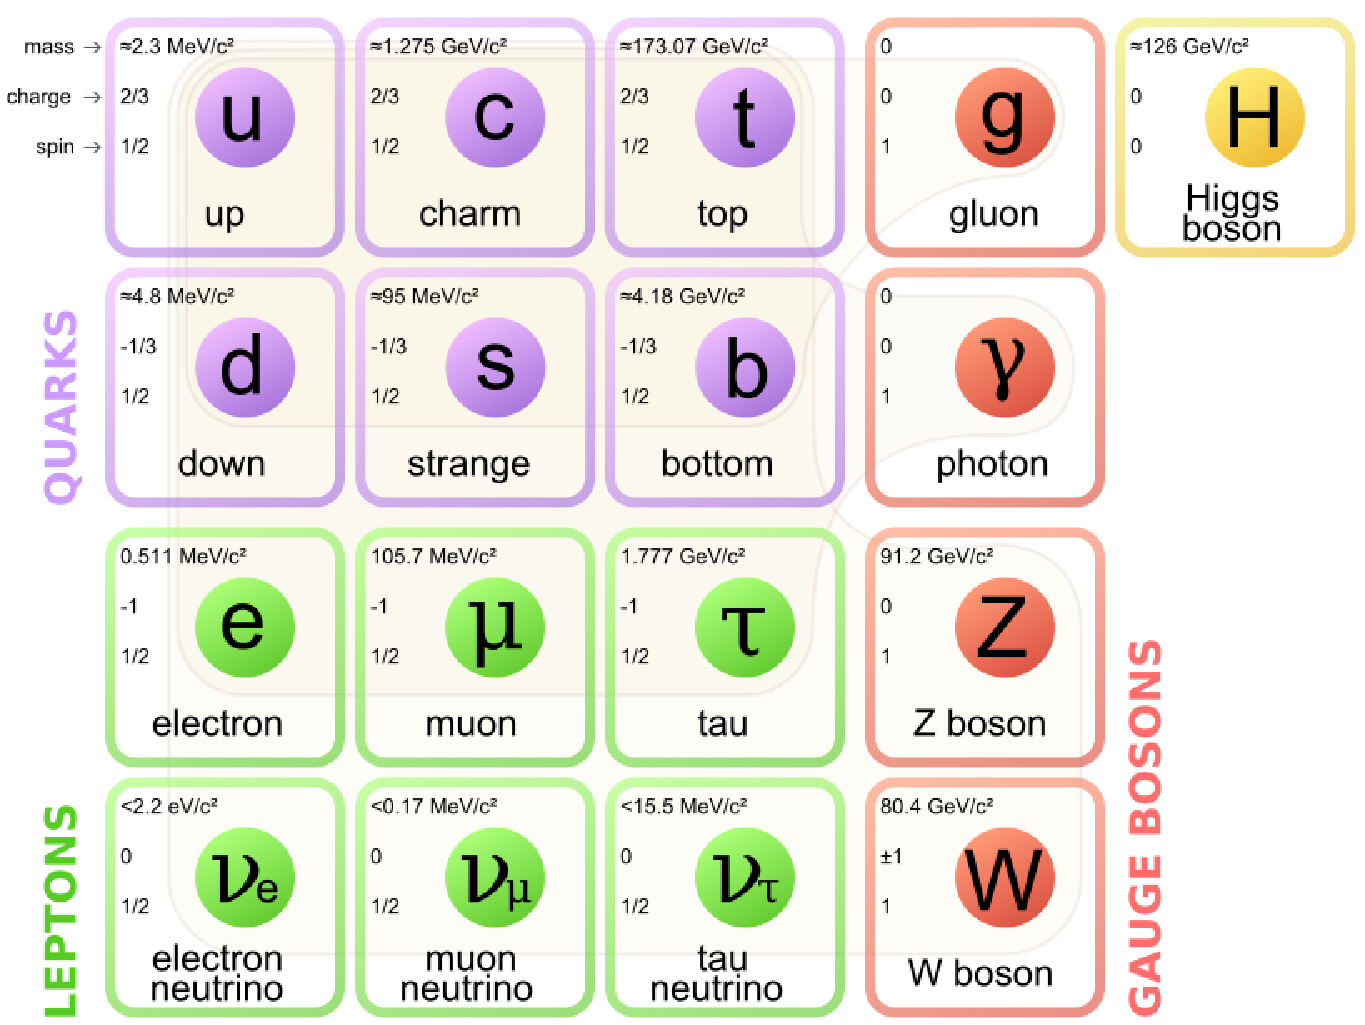
\includegraphics[width=10cm]{chap0/Standard_Model_of_Elementary_Particles.pdf}
  \caption{标准模型中的基本粒子}
  \label{fig:standard_model_particle}
\end{figure}

粒子物理学是一门实验科学。粒子物理实验的主要手段有宇宙线,高能物理加速器和粒子探测器~\cite{tangxw1982}~\cite{xukz1981}~\cite{xieyg2003}\cite{xuefj2003}。研究越深层次的物质结构需要越精细的探针:即更高能量的入射粒子。高能加速器具有高能量,高亮度的特点,可以控制产生粒子物理实验所需要的高能粒子束流。

加速器物理实验通过粒子加速器把带电粒子加速到很高的能量,之后通过对撞或者打靶让高能粒子之间(对撞机实验)或者高能粒子和其他物质之间(固定靶实验)发生相互作用,通过一系列的探测器测量碰撞后的产生的次级粒子各类信息,借助必要的分析方法和研究手段,进而研究它们的性质和相互作用规律。对撞机实验和固定靶实验是加速器物理实验的两种方式,它们各有利弊。对撞机实验的优点是加速器的束流能量能够被完全的利用,缺点是束流种类、反应末态和对撞亮度等均受到限制。固定靶实验的优点是可以使用的束流和粒子种类多,反应的末态也比较丰富,但缺点是束流的能量不能完全的被利用。

对撞机实验在加速器实验中有着很重要的地位。~$J/\psi$~粒子、~$\tau$~轻子和~$\Upsilon$~粒子都可以在对撞实验中被发现,高能量的~$Z^{0}$~粒子、~$W^{\pm}$~粒子、t夸克和~higgs~粒子也都是在对撞实验中被发现的。表~\ref{tbl:collider-accelerator}~列出了世界上主要的加速器及其研究重点。

\begin{table}[h]
    \centering
    \caption{\label{tbl:collider-accelerator} 主要高能物理对撞机及其研究重点}
    \footnotesize
    \begin{tabular}{lllll}
        \hline
        名称& 国家& 粒子源& 能量(~Gev~)& 研究重点\\
        \hline
        BEPC(BEPCII)& 中国& $e^{+}$/$e^{-}$& 2~5& 粲夸克、$\tau$粲能区物理 \\
        CESR& 美国& $e^{+}$/$e^{-}$& 10& b夸克 \\
        CESR-c& 美国& $e^{+}$/$e^{-}$& 3-11& 粲偶素、D物理 \\
        HERA& 德国&  $e^{-}$/$\overline{p}$&30/820& 质子结构\\
        TEVATRON& 美国& p/p&1800& t夸克\\
        PEPII& 美国& $e^{+}$/$e^{-}$& 3.1/9& b介子、CP破坏\\
        KEKB& 日本&   $e^{+}$/$e^{-}$& 3.5/8& b介子、CP破坏\\
        RIHC& 美国& $A_{u}$/$A_{u}$& 200& 重离子对撞\\
        LHC& 瑞士(CERN)& p/p(Pb/Pb)& 14000(2700)& Higgs、b介子、CP破坏、重离子\\
        \hline
    \end{tabular}
\end{table}

北京正负电子对撞机~\cite{xiejl1996}~\cite{ihep:2003}~\cite{ihep:2006}实验取得了一系列重要的物理成果,其中包括:~$\tau$~轻子质量的精确测量、~2-5Gev~强子反应界面的精确测量、~X(1835)~共振态的发现和~$Z_{c}(3900)$~\cite{BESIII:2013}共振态的发现等。

\section{北京正负电子对撞机~(BEPCII)~}

坐落于北京西郊的北京正负电子对撞机(Beijing Electron Positron Collider,~BEPC)及其配套装置北京谱仪~\cite{zhengzp2009}(Beijing Spetrometer,~BES)建于~1988~年。1994~-~1996~年,对撞机进行过升级改造仍旧称作~BEPC,此时谱仪则称为~BESII。
图~\ref{fig:bepc}~给出了北京正负电子对撞机鸟瞰图示意图。
\begin{figure}[!h]
  \centering
  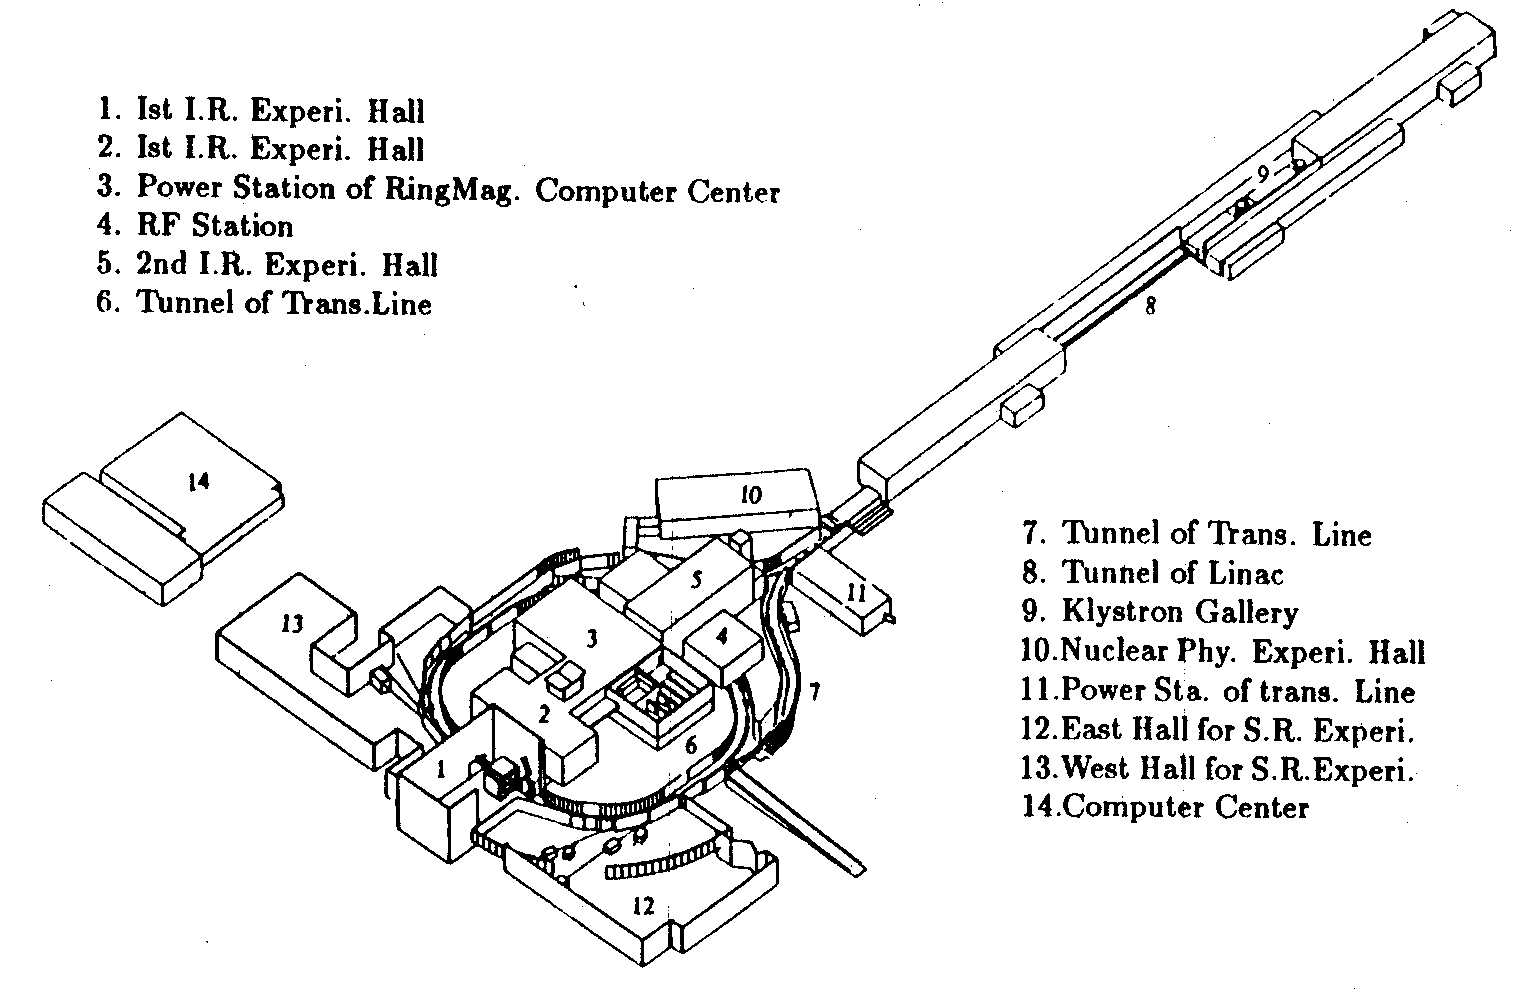
\includegraphics[width=10cm]{chap0/bepc.png}
  \caption{北京正负电子对撞机鸟瞰图}
  \label{fig:bepc}
\end{figure}

2004~年到~2008~年,BEPC~和~BESII~完成升级改造,升级后的对撞机称为~BEPCII,谱仪称为~BESIII~\cite{M.A:2010}。%升级后~BEPCII~和~BESIII~一直运行稳定。
表~\ref{tbl:BEPCII-VS-BEPC}~列出了~BEPCII~主要设计参数。
\begin{table}[htp]
  \centering
  %\footnotesize
  \caption{\label{tbl:BEPCII-VS-BEPC} BEPCII~和~BEPC~主要设计参数比较}
  \begin{tabular}{ccc}
    \hline\hline
    参数 & BEPCII & BEPC \\
    \hline
    质心能量~(GeV) & 2-4.6 & 2-5 \\
    储存环长度~(m) & 237.5 & 240.4 \\
    环的数目 & 2 & 1 \\
    高频频率~$f_{rf}$~(MHz) & 499.8 & 199.5 \\
    $2\times1.89$~GeV~(cm$^{-2}$s$^{-1}$)~下的峰值亮度 & $\sim10^{33}$ & $\sim10^{31}$ \\
    束团个数 & 2 & 1 \\
    束团流强~(A) & $2 \times 0.91$ & $2 \times 0.035$ \\
    束团间隔~(m/ns) & 2.4/8 & - \\
    束团长度~($\sigma_z$)~cm & 1.5 & $\sim 5$ \\
    束团宽度~($\sigma_x$)~$\mathrm{\mu m}$ & $\sim380$ & $\sim840$ \\
    束团高度~($\sigma_y$)~$\mathrm{\mu m}$ & $\sim5.7$ & $\sim37$ \\
    相对能散 & $5 \times 10^{-4}$ & $5 \times 10^{-4}$ \\
    对撞点束流夹角~(mrad) & $\pm 11$ & 0 \\
    \hline\hline
  \end{tabular}
  \label{tab:bepciiParam}
\end{table}

\begin{comment}
升级后的~BEPCII~是一个多束团的双环对撞机。双环指的是正负电子束流分别注入在两个彼此独立的储存环中,经加速后在对撞点发生对撞。多束团对撞可以大幅度的提高亮度。~BEPCII~的峰值亮度设计为在~1.89Gev~处达~1$\times$$10^{33}$$cm^{-2}$$s^{-1}$。高亮度意味着可以获得大量的物理事例,为诸多基于巨大统计量的物理过程的研究和分析提供良好的实验基础。表~\ref{tbl:event-Number}~列出了~BEPCII~运行一年可以累积的各种物理事例数。
\begin{table}[h]
    \centering
    \caption{\label{tbl:event-Number} BEPCII运行一年可以积累的事例数}
    \footnotesize
    \begin{tabular}{llllc}
        \hline
        物理& 质心系能量& 峰值亮度& 物理截面& 每年产生事例数 \\
             &(Gev)      &($10^{33} $$cm^{-2}$$s^{-1}$)& (nb)\\
        \hline
        $J/\psi$& 3.097& 0.6& ~3400&  10$\times$$10^{9}$ \\
        $\tau$&   3.670& 1.0& ~2.4&    12$\times$$10^{6}$ \\
        $\psi'$&  3.686& 1.0& ~640&    3$\times$$10^{9}$\\
        D&        3.770& 1.0& ~6.5&    32$\times$$10^{6}$\\
        $D_{s}$&   4.040& 0.6& ~0.32&   1$\times$$10^{6}$\\
        $D_{s}$&   4.160& 0.6& ~1.0&    3$\times$$10^{6}$\\
        \hline
    \end{tabular}
\end{table}

\section{~BESIII~物理目标}
~BEPCII~运行在~$\tau$~-粲能区($\approx$~3~Gev),~BESIII~是运行在~BEPCII~上的大型通用探测器,通过收集~$\tau$~-粲能区的正负电子对撞产生的末态粒子进行~$\tau$~-粲物理研究。~BESIII~主要研究的物理目标有:轻强子谱、粲物理、~QCD~与~$\tau$~物理~\cite{wangyf2011}~\cite{chaokt:2009}。
\end{comment}

\section{北京谱仪(BESIII)的物理目标}
北京正负电子对撞机运行在$\tau$-粲能区,升级后~BEPCII~峰值亮度与之前的~BEPC~相比提高了~100~倍,即每秒可以获取的事例数提高了~100~倍,BESIII~是与此高亮度相对应的高精度探测器,可以为该能区的物理研究的高精度测量提供良好的条件。

BEPCII~的峰值亮度设计为在~1.89~Gev~处达到~1$\times$$10^{33}$$cm^{-2}$$s^{-1}$(已于~2015~年~4~月~5~日成功达到),是$\tau$-粲能区历史上的最高值,获得了大量物理事例,提供了得到重要物理结果的机会。综合加速器的亮度、运行时间、各类事例的产生截面、探测器的最大覆盖立体角及正负电子束流的能散度,BEPCII~一年运行取数中各种事例数的列表~\cite{yuancz:2002}~见表~\ref{tbl:event-Number}~

\begin{table}[h]
    \centering
    \caption{\label{tbl:event-Number} BEPCII运行一年可以积累的事例数}
    \footnotesize
    \begin{tabular}{llllc}
        \hline
        物理& 质心系能量& 峰值亮度& 物理截面& 每年产生事例数 \\
             &(Gev)      &($10^{33} $$cm^{-2}$$s^{-1}$)& (nb)\\
        \hline
        $J/\psi$& 3.097& 0.6& ~3400&  10$\times$$10^{9}$ \\
        $\tau$&   3.670& 1.0& ~2.4&    12$\times$$10^{6}$ \\
        $\psi'$&  3.686& 1.0& ~640&    3$\times$$10^{9}$\\
        D&        3.770& 1.0& ~6.5&    32$\times$$10^{6}$\\
        $D_{s}$&   4.040& 0.6& ~0.32&   1$\times$$10^{6}$\\
        $D_{s}$&   4.160& 0.6& ~1.0&    3$\times$$10^{6}$\\
        \hline
    \end{tabular}
\end{table}

结合考虑~BESIII~探测器的性能和具体可以获取的各类事例数,BESIII~的物理研究目标为:轻强子谱、粲偶素物理、粲物理、QCD与~$\tau$~物理等,黄皮书~Physics at BESIII~里给出了~BESIII~详细的物理目标。~\cite{chaokt:2009}~\cite{wangyf2011}~

\section{~BESIII~探测器}
北京谱仪是各种粒子探测器的组合,通过对正负电子对撞后产生的次级带电粒子的动量、能量、位置、质量等各种参数的观察和测量,重建各类反应过程,进而研究物质的基本性质。~BEPCII~的特点是高亮度、多束团,其设计亮度是~BEPC~的~100~倍,高亮度意味高统计量,这样~BESIII~的统计误差只有~BESII~的近~1/10~,对撞机的高性能和实验的高精度要求都需要有一个高质量的~BESIII~探测器。因此~BESIII~探测器既需要满足多束团、高计数率下的取数要求,同时探测器的系统误差也应该减少到之前~BESII~的~1/10~下。基于此,~BESIII~的设计必须满足以下要求:
\begin{itemize}
\item{10MeV~到~2.5Gev~内,有良好的能量分辨率,位置分辨率和光子鉴别能力;}
\item{50Mev~到~2.5Gev~内,能精确的测量带电粒子的动量和方向;}
\item{50Mev~到~2.5Gev~内,有好的粒子鉴别能力;}
\item{电子学系统和数据获取系统能够满足多束团模式和高数据率取数的要求。}
\end{itemize}

为满足以上要求,~BESIII~探测器的最终设计为:
\begin{itemize}
\item{径迹探测器选用的单丝分辨率好于~115$\mu$m~的小单元结构的氦基气体漂移室;}
\item{电磁量能器选用采用碘化铯(~$C_{s}$I~)晶体量能器,用来探测和鉴别光子和电子;}
\item{飞行时间探测器由塑料闪烁体构成,用来粒子鉴别;}
\item{超导螺线管磁铁的场强采用~1.0T~的;}
\item{~$\mu$~子室采用阻性板探测器;}
\item{前端电子学系统采用流水线技术,用来适应多束团模式和高数据率的数据获取系统。}
\end{itemize}

表~\ref{tbl:BESIII-VS-BESII}~列出了~BESIII~各组成部分的主要性能。
\begin{table}[h]
	\centering
	\caption{\label{tbl:BESIII-VS-BESII} BESIII~和~BESII~探测器的比较}
    \scalebox{0.8}{
	%\footnotesize
	\begin{tabular}[c]{llll}
		\hline
		子系统&  ~BESIII(当前指标)~&   ~BESIII(设计指标)~& ~BESII~ \\
		\hline
        \multirow{3}{4cm}{主漂移室}& $\sigma_{xy}$~=~115~ $\mu$m& $\sigma_{xy}$~=~130~ $\mu$m & 250~$\mu$m \\
                &  &   $\Delta$p/p = 0.5~$\%@$1~Gev&  2.4~$\%$@1~Gev \\
                & $\sigma_{dE/dx}$~$<$~5~$\%$ &  $\sigma_{dE/dx}$ = 6~$\%$&      8.5~$\%$       \\
        \hline
        \multirow{2}{4cm}{电磁量能器}&   $\sigma_{E}$/E = 2.4~$\%@$1~Gev& $\sigma_{E}$/E = 2.5~$\%@$1~Gev&  20~$\%$@1~Gev \\
                  & &   $\sigma_{x,y}$ = 0.6~cm@1~Gev&   3~cm@1~Gev \\
        \hline
        \multirow{2}{4cm}{飞行时间探测器}&   $\sigma_{T}$=68~ps(桶部)& $\sigma_{T}$=100~ps(桶部)& 180~ps(桶部)\\
                    & &  $\sigma_{T}$=110~ps(端盖)& 350~ps(端盖)\\          
        \hline
        $\mu$子计数器& &  9~层& 3~层  \\
        \hline
        磁铁& & 1.0T~& 0.4~T\\
		\hline
	\end{tabular}
    }
\end{table}

%图~\ref{fig:BESIII}~给出了BESIII总体结构端面视图。
\begin{figure}[!h]
  \centering
  \includegraphics[width=10cm,angle=90]{chap0/bes_view.eps}
  \caption{~BESIII~总体结构端面视图}
  \label{fig:BESIII}
\end{figure}
图~\ref{fig:BESIII}~给出了北京谱仪总体结构端面视图。
由内到外分别是:束流管~(Beam Pipe)~,主漂移室~(Main Drift Chamber,MDC)~,飞行时间探测器~(Time of Flight Counter,TOF)~,电磁量能器~(Electromagnetic Calorimeter,EMC)~,超导磁铁~(Superconducting Magnet,SM)~,~$\mu$~子探测器。
此外,~BESIII~还具有用于监视谱仪各部分的运行并记录其运行参数的分布式的慢控制系统~(slow control system)~;高保真读出各探测器信号的电子学系统~(read-out electronics system)~;在线选择感兴趣的事例的触发系统~(trigger system)~;在线数据获取系统~(data acquisition system,DAQ)~,以及用于处理记录下来的数据的离线数据系统~(offline data processing system)~。
%\subsection{主漂移室(Main Drift Chamber)}
\subsection{主漂移室}
主漂移室的主要任务是:

\begin{itemize}
\item{完成从对撞点产生的带电粒子动量和方向的精确测量;}
\item{完成电离能损~(dE/dx)~测量,用作带电粒子的粒子鉴别;}
\item{对带电粒子的测量提供尽可能大的立体角覆盖~(~97$\%$ 4$\pi$)~}
\item{带电粒子在低动量时,径迹重建也有足够高的效率;}
\item{提供带电粒子的一级硬件触发信号。}
\end{itemize}

%主漂移室的主要任务:为$\tau$-charm能区产生的带电粒子提供优秀的动量测量能力,同时提供好的电离能损的测量能力;
%提供一级触发的信号,用来筛选好的物理事例,压缩本底。

主漂移室中带电粒子的动量测量依赖于其在漂移室中径迹的测量,带电粒子在漂移室中击中的丝层越多,击中位置越多,径迹重建出来的粒子的飞行轨迹就越确定,测得的动量也就越准确。带电粒子在飞行过程中与探测器中的物质发生的多次库仑散射效应是影响低动量带电粒子动量测量精度的主要因素。为减少多次库仑散射的影响,漂移室的气体和场丝需要尽可能的选用低原子序列的材料。

漂移室采用小单元结构,场丝使用镀金铝丝,工作气体为~$H_{e}$/$C_{3}H_{8}$(60/40)~。立体角覆盖~$\Delta\Omega/4\pi$=0.93~,单丝的位置精确度为~130$\mu$m~.对于动量为~1~Gev~的带电粒子动量分辨率为~0.5~$\%$左右;在粒子的入射角为~$90\degree$~,~dE/dx~分辨~6~$\%$下,~$\pi/K$~的分辨能力(3$\sigma$)可达到~770~Mev/c。
\begin{figure}[!h]
  \centering
  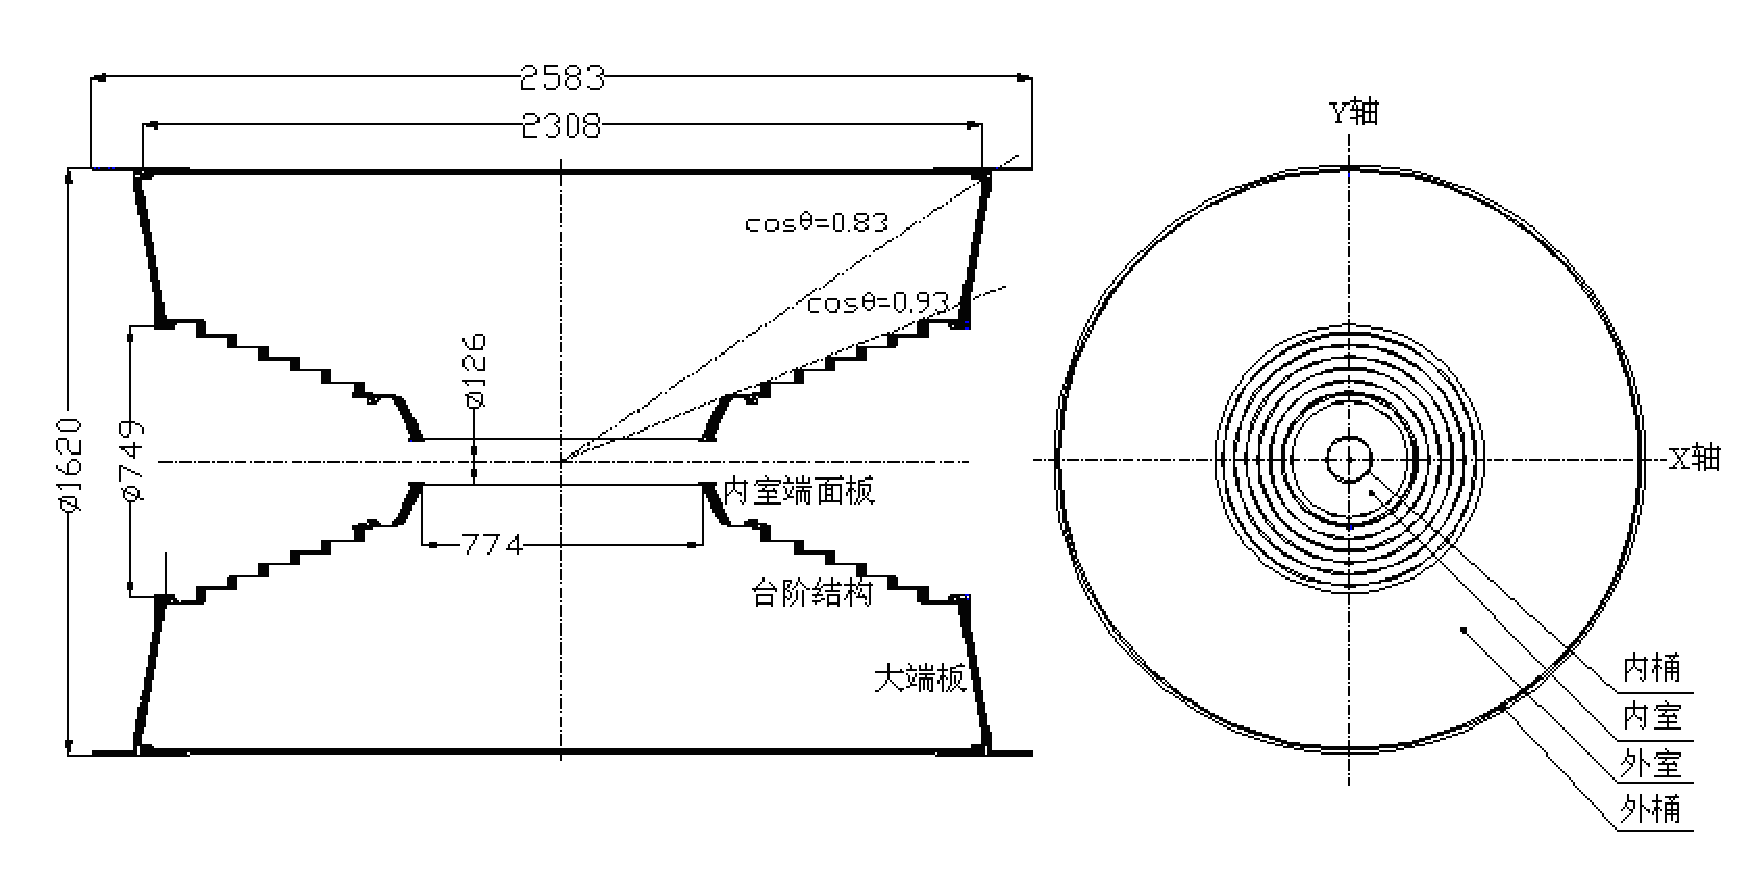
\includegraphics[width=10cm]{chap0/mdc-global.eps}
  \caption{主漂移室的结构示意图}
  \label{fig:mdc-global}
\end{figure}
%图~\ref{fig:mdc-global}~给出了MDC的结构示意图。

%\subsection{飞行时间探测器(Time of Flight Counter)}
\subsection{飞行时间探测器}
粒子鉴别是BESIII~的飞行时间探测器主要目的。决定其鉴别能力大小是相同动量的不同种类的带电粒子的飞行时间差和其自身的时间分辨率。
飞行时间探测器由桶部飞行时间探测器和端盖飞行时间探测器构成。其中,桶部部分固定在主漂移室上,采用双层结构,每层~88~块,共~176~块。每块长~2.32~m,厚~5~cm,梯形截面。信号由双端读出。端盖固定在端盖电磁量能器上,有东西两部分,每部分~48~个扇形闪烁体。桶部的立体角覆盖为~$|$cos($\theta$)$|<$0.83~;端盖的立体角覆盖为~0.85$<|$cos($\theta$)$|<$0.95~;桶部的时间分辨设计指标是~100~ps,在粒子的入射角为~$90\degree$~,~$\pi/K$~的鉴别能力~(3$\sigma$)~大约达到~700~Mev/c。

%\subsection{电磁量能器(Electromagnetic Calorimeter)}
\subsection{电磁量能器}

电磁量能器可以精确测量的光子的能量和提供触发中性事例的信号。在动量大于~200~Mev/c下有好的~e/$\pi$~的分辨能力。EMC~有桶部和端盖部分组成,共有~6240~块晶体,其中桶部的内半径有~94~cm,内长~275~cm,覆盖角~$|$cos($\theta$)$|<$0.82~;端盖覆盖角为~0.83$<|$cos($\theta$)$|<$0.93~。EMC的能量覆盖范围为~20~Mev~~2~Gev,在~1~Gev下,能量分辨率为~$\Delta$E/$\sqrt E$=2.5$\%$~,位置分辨率为~$\sigma$=0.6cm/$\sqrt E$(E in Gev)~。
\begin{figure}[!h]
  \centering
  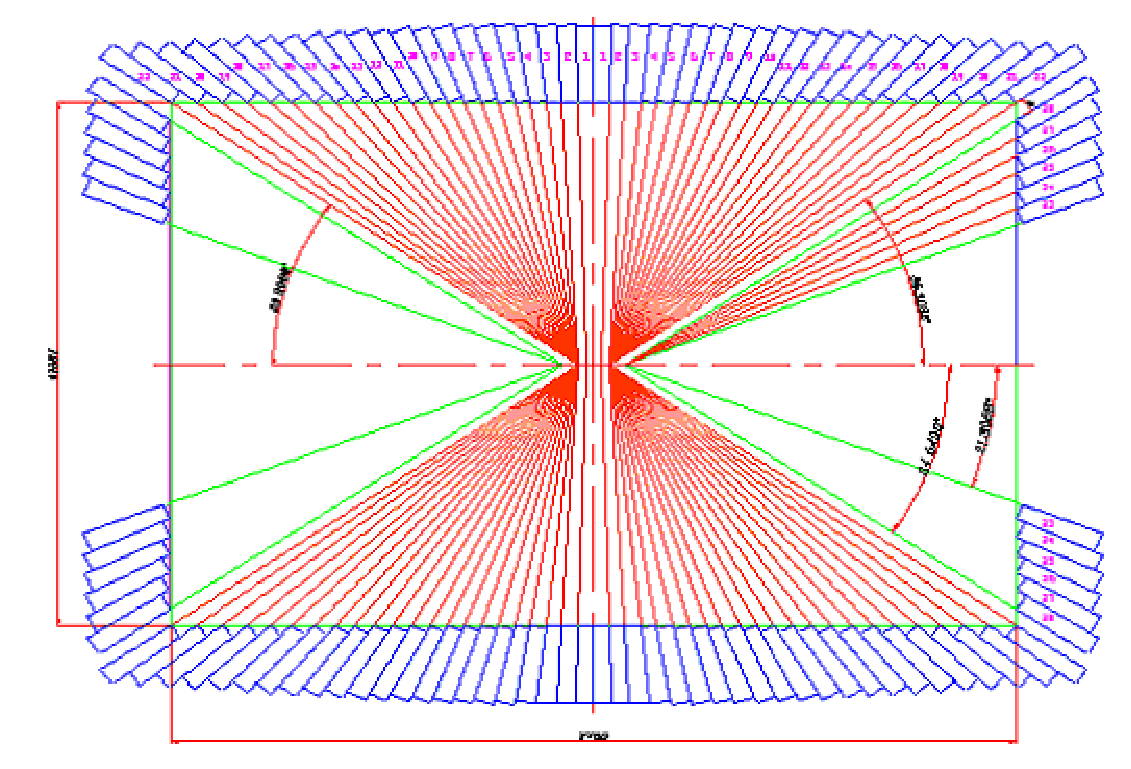
\includegraphics[width=10cm]{chap0/besiii-emc.eps}
  \caption{EMC晶体分布示意图}
  \label{fig:besiii-emc}
\end{figure}
%图~\ref{fig:besiii-emc}~给出了MDC的结构示意图。

\subsection{$\mu$子探测器}

位于BESIII探测器的最外层是~$\mu$~子探测器,有~$\mu$~子探测器和强子吸收体两个部分组成,从末态的带电粒子中区分出~$\mu$~子和$\pi$等其他带电强子是它的主要功能。~$\mu$~子探测器选用的是阻性板计数器(resistive plate counters,RPC)。为了增大立体角覆盖,~$\mu$~子探测器设计成桶部和端盖两部分。桶部~$\mu$~子探测器的内半径为~170~cm,外半径为~262~cm,共有8层按照八角形排列,厚度为~3-8~cm的RPC和吸收铁组成。吸收铁和~RPC~采用夹层结构,两层铁之间夹缝为~4~cm,~RPC~位于其中。端盖采用夹层结构,共计~8~层吸收铁和~8~层RPC相互夹层。桶部立体角覆盖最内层为~0.75~,最外层为~0.60~,总的桶部端盖立体角覆盖为~0.85~。在不同入射角度下,对于动量$>$~0.4~Gev的~$\mu$~子,探测效率均大于等于~95$\%$~。

%\subsection{超导磁铁(Superconducting Magnet)}
\subsection{超导磁铁}

超导磁铁是北京谱仪的一个重要组成部分,磁场回路选用的是轭铁,可以提供具有高强度的和一定均匀度的轴向磁场,带电粒子在此磁场中螺旋运动,可以供主漂移室测量带点粒子的径迹。磁铁长~4.91~m,内直径为~2.75~m,外直径为~3.4~m,中心直径为~2.95~m,线圈长度为~3.52~m。轭铁分为桶部和端盖两部分,除了作为磁场回路外,也做~$\mu$~子探测器的吸收体。磁场的强度越高,主漂移室中带电粒子的动量分辨率就越好,但同时磁场强度过高时,会不利于低动量的径迹测量。综合考虑,超导磁铁的中心磁场强度设计为沿束流方向为1.0T,主漂移室中磁场的不均匀性~不大于$5\%$~,测量的磁场精度不大于~$0.1\%$~。

\section{飞行时间探测器}

粒子的飞行时间是由飞行时间探测器测量出来的。具体来说,测量的是粒子到达飞行时间探测器的时刻。测量的时间和束流在对撞顶点发生对撞的时刻(~$t_{0}$~)之间的时间间隔,就是粒子从对撞点飞行到飞行时间探测器的时间。(见图~\ref{fig:TOF-theory}~,图~\ref{fig:traw}~)
%粒子鉴别正是利用得到的测量飞行时间结合利用主漂移室测量的粒子动量~p~和飞行径迹~$\L$~得到的预期飞行时间完成的。

%图~\ref{fig:TOF-theory}~给出了TOF探测器原理示意图。
\begin{figure}[!h]
  \centering
  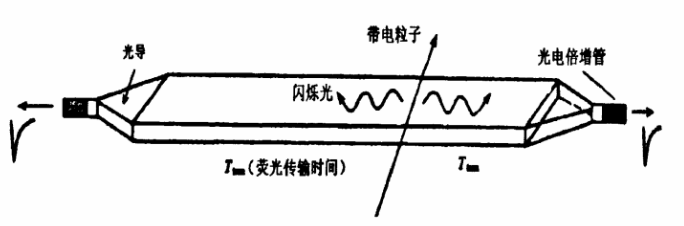
\includegraphics[width=0.9\textwidth]{chap0/TOF-theory.png}
  \caption{TOF探测器原理示意图}
  \label{fig:TOF-theory}
\end{figure}

\begin{figure}[!h]
  \centering
  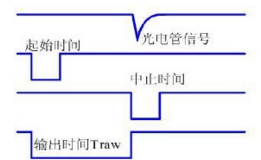
\includegraphics[width=0.5\textwidth]{chap0/traw.png}
  \caption{TOF探测器测量的飞行时间}
  \label{fig:traw}
\end{figure}

带电粒子从对撞顶点到击中~TOF~的预期飞行时间~$t_{exp}$~由公式~\ref{eq:0.1}~给出,其中~$L$~是带电粒子从对撞顶点到击中~TOF~的飞行距离。$\beta$~是带电粒子的飞行速度,由公式~\ref{eq:0.2}~给出,其中~m~是带电粒子的质量,~p~是带电粒子的动量。L~和~p~都是由主漂移室测量得到的。

\begin{align}
t_{exp}=L/\beta c 
\label{eq:0.1}\\
\beta=p/\sqrt {p^{2}+m^{2}}
\label{eq:0.2}
\end{align}

%由公式~\ref{eq:0.1}~和~\ref{eq:0.2}~即可求出粒子的质量$m_{0}$,鉴别出带电粒子。

对于动量都等于~p,质量分别为~$m_{1}$~和~$m_{2}$~的两个带电粒子,它们的飞行时间差的具体由公式~\ref{eq:0.4}~给出。
\begin{align}
\frac{1}{\beta^{2}_{2}}-\frac{1}{\beta^{2}_{1}}=\frac{m^{2}_{2}-m^{2}_{1}}{p^{2}}
\label{eq:0.3}\\
t_{2}-t_{1}=\frac{L}{c\beta_{2}}-\frac{L}{c\beta_{1}}=(\frac{L}{c})(\frac{m^{2}_{2}-m^{2}_{1}}{p^{2}})(\frac{\beta_{1}\beta_{2}}{\beta_{1}+\beta_{2}})\leq(\frac{L}{c})(\frac{m^{2}_{2}-m^{2}_{1}}{2p^{2}})
\label{eq:0.4}
\end{align}
由公式~\ref{eq:0.4}~可知,粒子飞行距离越长,粒子动量越小,则粒子的鉴别能力越好。

\subsection{粒子鉴别}
粒子鉴别是飞行时间探测器的主要物理目标,其鉴别能力的大小主要决定于相同动量的不同种类带电粒子的飞行时间差和飞行时间探测器自身的时间分辨所。它通过测量带电粒子在主漂移室内的飞行时间,结合主漂移室测得粒子的动量和径迹,根据不同粒子的质量不同,从而辨别粒子的种类;飞行时间探测器也参与第一级触发判选,不同探测器输出信号之间时间关系可以被用来排除宇宙线本底的影响。内半径越大,飞行时间探测器的飞行时间差越大;推算的对撞的事例起始时间精度和测量的带电粒子打到飞行时间探测器后的截止时间的精度分别决定时间分辨率,其中主要因素是飞行时间探测器自身的时间分辨率。

影响TOF的时间分辨的因素很多,总的时间分辨~$\sigma$~可以写成:
\begin{displaymath}
\sigma=\sqrt{\sigma_{TOF}^{2}+\sigma_{bunch-time}^{2}+\sigma_{bunch-length}^{2}+\sigma_{Z-position}^{2}+\sigma_{electronics}^{2}+\sigma_{expect}^{2}+\sigma_{time-walk}^{2}}
\end{displaymath}

其中~$\sigma_{TOF}$~是~TOF~的本征时间分辨率,反映了探测器的主要性能;~$\sigma_{bunch-time}$~表示对撞束团的时间不确定性;~$\sigma_{bunch-length}$~表示由于束团的长度引起的对撞时刻的不确定性;~$\sigma_{Z-position}$~来源于粒子击中闪烁体的沿束流方向位置的不确定性,会引起光信号在闪烁体内的传输时间不确定;~$\sigma_{electronics}$~表示来自电子学时间测量的不确定性;~$\sigma_{expect}$~表示来自预期飞行时间的不确定性;~$\sigma_{time-walk}$~表示来源于过阈时间的时间晃动效应。

表~\ref{tbl:TOF-expect-sigma}~列出了预期的~TOF~时间分辨率分析。
\begin{table}[h]
    \centering
    \caption{\label{tbl:TOF-expect-sigma} 预期的TOF时间分辨率分析}
    \footnotesize
    \begin{tabular}{lll}
        \hline
        时间分辨项目& 桶部时间分辨率& 端盖时间分辨率 \\
        \hline
        单层TOF本征时间分辨率(对1Gev的$\mu$子)& 80-90ps&        80ps \\
        束团时间的不确定性&                     5ps&            5ps \\
        束团长度的不确定性&                     15mm,35ps&      15mm,35ps\\
        MDC外推的定位精度&                      5mm,33ps&       5-10mm,47-95ps\\
        电子学测量的精度&                       25ps&           25ps\\
        预期飞行时间精度&                       30ps&           40ps\\
        时幅修正&                               10ps&          10ps  \\
		单层TOF总的时间分辨率&                   100-110ps&     110-137ps           \\
		双侧TOF总的时间分辨率&                   80-90ps&       无                \\       
        \hline
    \end{tabular}
\end{table}

\subsection{桶部TOF和端盖TOF}
桶部~TOF~的径向半径从~810~mm到~925~mm。桶部闪烁体选用的是长度为~2.3~m,宽度约为两英寸,厚度为~5~cm,型号为~BC408~闪烁体。
%图~\ref{fig:TOF}~给出了~TOF~的结构示意图。
\begin{figure}[!h]
  \centering
  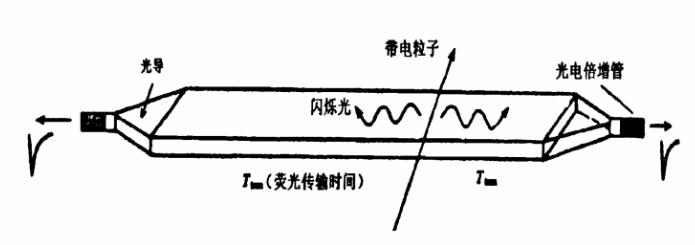
\includegraphics[width=0.8\textwidth]{chap0/TOF.png}
  \caption{飞行时间探测器结构 BTOF指的桶部TOF,ETOF指的端盖TOF}
  \label{fig:TOF}
\end{figure}

端盖TOF的塑料闪烁体的长度短于桶部~TOF~,选用的是~BC404~信号的闪烁体,可以充分发挥~BC404~光产额高,时间快的优势。
\begin{figure}[!h]
  \centering
  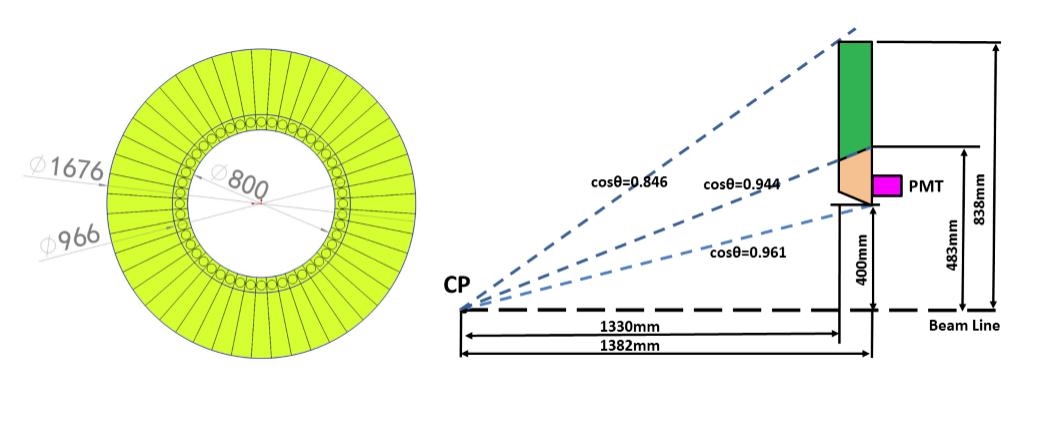
\includegraphics[width=0.9\textwidth]{chap0/ETOF.png}
  \caption{端盖TOF几何尺寸与空间安排}
  \label{fig:ETOF}
\end{figure}
%图~\ref{fig:ETOF}~给出了ETOF的结构示意图。
\subsection{TOF的电子学系统}
飞行时间探测器的电子学系统的基本功能是对带电粒子的飞行时间进行测量。简单讲,测量的是正负电子从对撞时刻到次级带电粒子击中飞行时间探测器刻度之间的时间间隔。快前沿定时是现代粒子物理实验测量时间最有效的定时方法。系统还需要对输出信号的幅度(电荷)进行测量,用来校正前沿定时方法中时间游走(time-walk)效应带来的测量误差。飞行时间探测器的还有一个主要功能是给触发系统提供粒子击中的快时间响应信号。
基于此,飞行时间探测器的电子学系统需要完成三项基本功能:时间测量,电荷测量,提供粒子击中的快时间响应。

TOF~的读出电子学系统由前置放大器部分和读出电子学~VME(Versa Module Eurocard bus Crate)系统组成。前置放大器对光电倍增管输出的探测器信号进行~10~倍的放大,输出的差分信号经过~18~米长的差分屏蔽电缆送入到读出电子学系统进行数字化处理。

TOF~前端电子学系统采用的是~VME$\quad$9U~作为~TOF~前端读出电子学系统的硬件平台;采用全差分的信号处理和传输技术;对时间和电荷量的测量采用统一的数字化处理。时间测量采用的是快前沿定时甄别+高性能时间数字转化器(high performance time to digital converter,HPTDC)~数字化技术。~TOF~采用阈值甄别技术,只有高于阈值的信号才能被电路输出。~HPTDC~时间测量直接测量的是粒子到达探测器的击中时间。飞行时间需要测量时间减去粒子对撞的初始时间得到。而粒子对撞的初始时间需要离线数据分析,找到对撞时间所对应的的时钟信号,然后结合束团之间固有的时间关系计算出来。

\section{论文选题的意义}

BESIII~实验的原始数据以二进制文件的形式记录并储存,记录的是在线数据获取系统经过触发判选以及在线选择的好事例。原始数据主要包含的信息量是探测器的电子学信号的时间和幅度信息。这样的原始数据是不能直接被物理分析使用的。原始数据需要经过一定的处理才能得到物理分析所需要的包括能量,动量,运动方向等的信息。这些需要的中间处理过程就是离线刻度和重建。离线数据刻度可以消除实验中的各种外部条件和探测器自身条件对电子学信号和物理测量量之间转化带来的影响。离线数据刻度对每个不同的子探测器分别进行,分别生成刻度常数。重建就是利用刻度得到的刻度常数将原始的数据重建转化为粒子的动量,能量,运动方向等物理量,生成重建数据。物理分析就是利用重建数据进行的。~\cite{wangyf2011}

BESIII实验在2015年夏季完成端盖飞行时间探测器的升级改造,用多气隙电阻性板室(Multi-gap Resistive Plate Chamber,简称MRPC)替代现有的闪烁体。MRPC~探测器具有较小的时间分辨,同时又能保证足够的探测效率。为与探测器硬件升级相适应,离线数据处理和分析系统需要完成~MRPC~端盖~TOF~的软件开发和数据处理方面的研究。

对端盖~MRPC-TOF~探测器的刻度方法进行研究,建立一套稳定并行之有效的刻度流程,满足数据刻度和重建的需要,把优秀的探测器指标转化为物理分析中的优良的粒子鉴别能力,是论文研究的主要内容,也是意义所在。
研究采用了样条插值和构造公式两种方法。之后的章节会详细探讨两种方法在新的~MRPC~飞行时间探测器离线数据刻度中的应用,以及在研究中遇到的难点及解决办法。

\section{MRPC刻度方法国内外现状}

相对论重离子对撞机~RHIC~是美国布鲁克海文国家实验室~(BNL)~的对撞机,其上的螺旋径迹探测器~STAR~实验~\cite{ruanlj:2005}~\cite{wuj:2005}~\cite{wangy:2010}的主要科学目标是寻找可能存在的新物质形态夸克-胶子等离子体,并研究极端高温、高密下的强相互作用物质的演化动力学。欧洲核子中心(CERN)的大型强子对撞机~LHC~上的大型离子对撞机~ALICE~实验~\cite{A.Alici:2012}~\cite{A.Alici:2014}是在极端能量密度下研究强相互作用物理,寻找夸克胶子等离子体,研究量子色动力学。这两个实验都采用~MRPC~做为飞行时间探测器。

\begin{comment}
~STAR~的~TOF~由~3840~块~MRPC~组成,每块有~6~个读数条。刻度样本选择的是动量在~0.3—0.6Gev/c~的~$\pi$~介子。由于信号在读出条内的反射,每个电子学读出通道的~TOT~(time-over-threshold~\cite{Shao:2009aa},简称TOT)分布存在多峰,且各不相同,时幅修正的刻度采用样条拟合(spline-fit)的方法。信号在读出条上的传输时间依赖信号传播距离,击中位置的修正只考虑沿读出条方向的效应。扣除起始时间晃动~55~ps后,时间分辨为~75~ps~\cite{Shao:2009aa}。

~ALICE~的~TOF~由~1593~块~MRPC~组成,每块面积为~7.4~cm$\times$~120~cm,每个模块~96~个读出端,每个读出端面积为~2.5~cm$\times$~3.5~cm。刻度样本需要完整的径迹重建。~TOF~刻度分为三个步骤:(1)一个整体的偏移;(2)每个电子学通道的偏移;(3)每个电子学通道的时幅修正。时幅修正采用的是~TOT~的~5~阶多项式拟合。扣除事例起始时间的影响后,时间分辨为~80~ps~\cite{A.A:2005}。
\end{comment}

\subsection{STAR~实验的~MRPC~飞行时间探测器离线数据的刻度方法}
\begin{figure}[!h]
  \centering
  \includegraphics[width=0.9\textwidth]{chap0/STAR-MRPC.png}
  \caption{STAR实验的MRPC模块结构图。(a)长边视图;(b)短边视图}
  \label{fig:STAR-MRPC}
\end{figure}

STAR~实验的圆柱型~TOF~覆盖面积大约有64$m^{2}$,整个系统由~120~个托盘,每个托盘有~32~个~MRPC~模块组成,每个~MRPC~模块有~6~个读数条。每个读数条长~6.0~cm,宽~3.1~cm~\cite{wangy:2010}。图~\ref{fig:STAR-MRPC}~给出了~STAR~实验的~MRPC~模块的结构图。实验采用基于~CERN~开发的~NINO~芯片的前端电子学系统,高性能的时间-数字转化电路(high-performance time to digital convertor,HPTDC)可以同时测量信号过阈的前沿和后沿时间。其中前沿时间用于定时,后沿时间和前沿时间之间的间隔为过阈时间(time-over-threshold,TOT),用于对前沿时间的晃动进行校准。

STAR~关于~MRPC-TOF~的刻度方法分为5步:
\begin{itemize}
\item{挑选样本:选择动量在~0.3-0.6~Gev $c^{-1}$,dE/dx$\textless~2.5~KeV cm^{-1}$的$\pi$(纯度$\geq99$$\%$)}
\item{对事例起始时间进行修正,按每个读出通道进行修正}
\item{对过阈时间进行修正,按每个读出通道进行修正}
\item{对击中读数条的位置进行修正,因为每个读数条信号的传播速度并不一致,按每个读出通道进行修正。(这里只考虑沿着读数条传播方向的效应)}
\item{对第三步和第四步进行第二次修正,进一步提高修正效应}
\end{itemize}

具体每步修正采用的是样条插值(spline fit)的方法。
图~\ref{fig:STAR-TOT}~是~STAR~实验测得的不同模式的过阈时间的分布。左边的图和中间的图可以看出很明显的多峰现象(这一点和我们~BESIII~的~MRPC~测得的过阈时间的分布很类似,都存在多峰现象)。
\begin{figure}[!h]
  \centering
  \includegraphics[width=0.9\textwidth]{chap0/STAR-TOT.png}
  \caption{STAR~实验测得的不同模式的过阈时间的分布。前两幅图可以明显看出多峰现象}
  \label{fig:STAR-TOT}
\end{figure}

图~\ref{fig:STAR-time}~是~STAR~实验测得的不同过阈时间模式下的原始时间的分布。
\begin{figure}[!h]
  \centering
  \includegraphics[width=0.9\textwidth]{chap0/STAR-time.png}
  \caption{HPTDC~测量的原始时间的分布。分别对应上图不同的过阈时间模式}
  \label{fig:STAR-time}
\end{figure}

图~\ref{fig:STAR-fit-TOT}~是~STAR~实验对过阈时间修正的方法,对于不同的过阈时间模式采用的都是样条插值的方法。
\begin{figure}[!h]
  \centering
  \includegraphics[width=0.9\textwidth]{chap0/STAR-fit-TOT.png}
  \caption{对应不同模式的过阈时间的样条插值}
  \label{fig:STAR-fit-TOT}
\end{figure}

图~\ref{fig:STAR-fit-t0}~表示插值拟合对事例起始时间的修正(这个修正放在修正过阈时间和击中位置之前的)。图~\ref{fig:STAR-fit-z}~表示插值拟合对击中位置的修正。
\begin{figure}[!h]
\begin{minipage}[!h]{0.48\linewidth}
\centering
\includegraphics[width=0.8\textwidth]{chap0/STAR-fit-t0.png}
\subcaption{插值方法拟合起始时间}
\label{fig:STAR-fit-t0}
\end{minipage}
%\hfill
\begin{minipage}[!h]{0.48\linewidth}
\centering
\includegraphics[width=0.8\textwidth]{chap0/STAR-fit-z.png}
\subcaption{插值方法拟合击中位置}
\label{fig:STAR-fit-z}
\end{minipage}%
\caption{插值方法拟合事例起始时间和击中位置}
\end{figure}


\begin{figure}[!h]
  \centering
  \includegraphics[width=0.9\textwidth]{chap0/STAR-res.png}
  \caption{最终修正后得到的时间分辨 (a)总的时间分辨;(b)每个道的时间分辨}
  \label{fig:STAR-res}
\end{figure}

图~\ref{fig:STAR-res}~是~STAR~实验修正后得到的时间分辨(过阈时间和击中位置都是修正了两次),约~89~ps,扣除起始时间的晃动(~55~ps),最终的MRPC的时间分辨是~75~ps。


\subsection{ALICE~实验的~MRPC~飞行时间探测器离线数据的刻度方法}
~ALICE~的~TOF~由~1593~块~MRPC~组成,每块面积为~7.4~cm$\times$~120~cm,每个模块~96~个读出端,每个读出端面积为~2.5~cm$\times$~3.5~cm。刻度需要完整的径迹重建。~TOF~刻度分为三个步骤:(1)一个整体的偏移;(2)每个电子学通道的偏移;(3)每个电子学通道的时幅修正。

图~\ref{fig:ALICE-offset}~对应上面的前两步。左图表示的是一个整体的偏移情况,右图表示的是拟合获取单个电子学通道偏移值。
\begin{figure}[!h]
  \centering
  \includegraphics[width=0.9\textwidth]{chap0/ALICE-offset.png}
  \caption{左图:LHC实验在2012年整体的电子学通道的时间偏移情况;右图:一个电子学通道的时间偏移的拟合}
  \label{fig:ALICE-offset}
\end{figure}

图~\ref{fig:ALICE-fit-TOT}~对应第三步的修正。其中对于时幅修正采用的是多项式拟合。
\begin{figure}[!h]
  \centering
  \includegraphics[width=0.9\textwidth]{chap0/ALICE-fit-TOT.png}
  \caption{时幅修正。径迹选择的是0.5$<$p$<$1.5Gev。上方:空的直方图和阴影的直方图分别表示拟合后和之后前的情况;下方:4个对数条拟合时幅修正的情况,采用的是多项式拟合}
  \label{fig:ALICE-fit-TOT}
\end{figure}

图~\ref{fig:ALICE-res}~对应第三步的修正。选择的是动量在0.95$<$p$<$1.05Gev/c范围内的~$\pi$~介子作为刻度样本。扣除起始时间的晃动后时间分辨是~80~ps。
\begin{figure}[!h]
  \centering
  \includegraphics[width=0.9\textwidth]{chap0/ALICE-res.png}
  \caption{ALICE实验的MRPC的时间分辨;选择的是动量在0.95$<$p$<$1.05Gev/c范围内的~$\pi$~介子作为刻度样本}
  \label{fig:ALICE-res}
\end{figure}

\section{论文的结构}
根据论文的主要内容,论文的结构安排如下:

第一章是论文的前言部分,简单介绍了粒子物理学和~BESIII~实验的基本知识,然后介绍了论文选题的背景和意义,以及国内外关于~MRPC~飞行时间探测器离线数据刻度方法。

第二章介绍了~BESIII~实验的~MRPC~端盖~TOF~,刻度重建流程,以及刻度中的重点和难点问题。

第三章介绍利用插值方法对~BESIII~的~MRPC~端盖~TOF~进行离线数据刻度的研究。

第四章介绍利用构造公式对~BESIII~的~MRPC~端盖~TOF~进行离线数据刻度的研究。

第五章介绍利用双端数据采用插值和构造公式两种方法对~BESIII~的~MRPC~端盖~TOF~进行离线数据刻度的研究。

第六章介绍了刻度公式的适用性问题,以及过阈时间和击中位置关联项的问题研究。

第七章对论文的内容进行总结。











